% Main entry point. Build here with: latexmk -pdf proposal.tex
% Section text is editable LaTeX; UI concepts are embedded raster images.
\documentclass[11pt,a4paper]{article}
\usepackage[T1]{fontenc}
\usepackage[utf8]{inputenc}
\usepackage[margin=25mm,headheight=15pt,headsep=8mm,footskip=12mm]{geometry}
\usepackage{newtxtext,newtxmath,microtype}
\usepackage[table]{xcolor}
\usepackage{graphicx,booktabs,array,tabularx,enumitem,caption,float}
\usepackage{setspace,titlesec,fancyhdr,tikz,tocloft}
\usetikzlibrary{arrows.meta,positioning,calc}
\usepackage{hyperref,bookmark}
\definecolor{navy}{HTML}{000000}
\definecolor{teal}{HTML}{000000}
\definecolor{muted}{HTML}{404040}
\definecolor{pale}{HTML}{F5F5F5}
\definecolor{line}{HTML}{BFBFBF}
\definecolor{amber}{HTML}{404040}
\hypersetup{colorlinks=true,linkcolor=navy,citecolor=teal,urlcolor=teal,
 pdftitle={EventLens - Event Risk Research for Indices and Equities},
 pdfauthor={Franklin, Anthony, Owen and Sunny},
 pdfsubject={HKUST Final Year Project Proposal, 2026--2027}}
\urlstyle{same}
\setstretch{1.08}
\setlength{\parindent}{0pt}
\setlength{\parskip}{5pt}
\setlength{\emergencystretch}{2em}
\setcounter{tocdepth}{2}
\setcounter{secnumdepth}{2}
\titleformat{\section}{\Large\bfseries}{\thesection}{0.7em}{}
\titleformat{\subsection}{\large\bfseries}{\thesubsection}{0.7em}{}
\titlespacing*{\section}{0pt}{0pt}{12pt}
\titlespacing*{\subsection}{0pt}{13pt}{5pt}
\setlist[itemize]{leftmargin=1.4em,itemsep=3pt,topsep=4pt,parsep=0pt}
\setlist[enumerate]{leftmargin=1.6em,itemsep=4pt,topsep=4pt,parsep=0pt}
\captionsetup{font=small,labelfont=bf,justification=raggedright,singlelinecheck=false,skip=7pt}
\renewcommand{\arraystretch}{1.16}
\setlength{\tabcolsep}{7pt}
\newcolumntype{L}[1]{>{\raggedright\arraybackslash}p{#1}}
\newcolumntype{Y}{>{\raggedright\arraybackslash}X}
\pagestyle{fancy}
\fancyhf{}
\fancyhead[L]{\small\sffamily\color{muted}EventLens}
\fancyhead[R]{\small\sffamily\color{muted}Final Year Project Proposal}
\fancyfoot[C]{\small\thepage}
\renewcommand{\headrulewidth}{0.3pt}
\fancypagestyle{plain}{\fancyhf{}\fancyfoot[C]{\small\thepage}\renewcommand{\headrulewidth}{0pt}}
\newcommand{\pagechapter}[1]{\clearpage\section{#1}}
\newcommand{\tablehead}{\rowcolor{pale}}
\newcommand{\smalltable}{\small\setstretch{1.04}}
\tikzset{flowbox/.style={draw=line,fill=pale,rounded corners=2pt,align=center,
 font=\small\sffamily,inner sep=7pt,minimum height=1.05cm},
 flowarrow/.style={-{Stealth[length=2mm]},draw=muted,line width=0.7pt}}
\renewcommand{\contentsname}{Table of Contents}
\renewcommand{\cftsecleader}{\cftdotfill{\cftdotsep}}
\setlength{\cftbeforesecskip}{7pt}
\setlength{\cftbeforesubsecskip}{2pt}
\setlength{\cftsecnumwidth}{2em}
\setlength{\cftsubsecindent}{2em}
\setlength{\cftsubsecnumwidth}{2.8em}
\patchcmd{\thebibliography}{\section*{\refname}}{}{}{}
\begin{document}
\thispagestyle{empty}
\vspace*{\fill}
\begin{center}
{\fontsize{40}{48}\selectfont\bfseries SW2\par}
\end{center}
\vspace*{\fill}

\clearpage
\thispagestyle{empty}
\vspace*{\stretch{2}}
\begin{center}
{\Huge\bfseries EventLens: Event Risk Research for\\[6pt] Indices and Equities\par}
\end{center}

\vspace*{\stretch{2}}
\begin{center}
by

\vspace{2mm}
Cheung Hau Yin Franklin \quad Anthony Hou \quad Liu Ngai Chiu \quad Sze Wang Cheong
\end{center}

\vspace*{\stretch{2}}
\begin{center}
Advised by \\
Prof. Shuai Wang
\end{center}

\vspace*{\stretch{2}}
\begin{center}
Submitted in partial fulfillment\\
of the requirements for COMP 4981 \\[2mm]
in the\\[2mm]
Department of Computer Science and Engineering\\
The Hong Kong University of Science and Technology
2026--2027
\end{center}

\vspace*{\stretch{2}}
\begin{center}
Date of submission: September 11, 2026
\end{center}

\vspace*{\stretch{1}}

\clearpage
\thispagestyle{empty}
\subsection*{Abstract}
EventLens is a proposed research dashboard that connects prediction-market events to the risks faced by investors in major US indices and a small selection of popular equities. A user will be able to find relevant events, compare the market's probability with a wallet-informed estimate, explore possible portfolio outcomes, and ask an AI assistant to explain the supporting evidence.

The central research question is whether a wallet's earlier forecasting record adds useful information beyond Polymarket prices and overall trading activity. We will combine market data, public blockchain records and equity-price histories, using only information available at each historical forecast time. Simple probability models will be evaluated first, followed by event-based portfolio scenarios and volatility forecasts. The initial event family will be US Federal Reserve rate decisions, subject to a data-feasibility review.

The prototype will cover three index-tracking exchange-traded funds and five selected equities, with cash available for paper portfolio comparisons. AI agents will retrieve evidence, request calculations from tested services and explain results. Numerical estimates will remain traceable to their data and model versions. Historical testing, data quality and user comprehension will determine success; improved prediction or profitable trading will be tested rather than assumed.

\clearpage
\pagenumbering{roman}
\tableofcontents
\clearpage
\pagenumbering{arabic}
\section{Introduction}
\subsection{Background and Motivation}
Financial markets are repeatedly repriced around discrete events such as central-bank decisions, elections, and geopolitical developments. Investors can observe news, asset prices, and volatility indicators, but these sources do not directly show a continuously updated probability of the underlying event. This project aims to develop an machine-learning-assisted quantitative analysis framework EventLensthat extracts information from prediction markets and evaluates its value in forecasting financial-market volatility. 

\textbf{Prediction markets.} Prediction markets such as Polymarket aggregate the beliefs of market participants into continuously updated probabilities. Market participants could trade YES and NO shares on the occurrence of events. A YES share pays one dollar if the specified outcome occurs and zero otherwise. A price of 60 cents can therefore be interpreted as an approximate market-implied probability of 60\% \cite{wolfers2004,wolfers2006}.

\textbf{Wallets and blockchain records.} Web 3 Prediction markets such as Polymarket records trade settlements on the blockchain. Its blockchain-based infrastructure provides transparent transaction histories that enable the behaviour and historical performance of individual participants (identified by their wallet addresses) to be analysed. This creates an opportunity to investigate whether information embedded in prediction-market activity, particularly from informed traders or "smart wallets", cancould provide useful signals for traditional financial markets.

\subsection{Objectives}
\begin{enumerate}
\item \textbf{Develop a smart-wallet identification model} using historical on-chain trading behavior to identify addresses whose decisions may add information beyond the market price.
\item \textbf{Construct smart-wallet-adjusted event probabilities} using wallet evidence and compare these experimental estimates with market-implied probabilities.
\item \textbf{Develop an event-to-asset relevance framework}: using statistical techniques and LLM research agent to identify traded events relevant to selected ETFs or indices.
\item \textbf{Evaluate whether Polymarket data provides incremental predictive valu} through historical backtesting and comparison against benchmark volatility forecasts, and present the results through an interactive AI-assisted dashboard
\end{enumerate}

The primary target user is a research-oriented retail investor or finance professional who understands basic portfolio concepts but lacks the infrastructure to query blockchains, evaluate prediction-market participants, and construct event-conditioned risk models. EventLens is intended as a research and paper-decision tool rather than personalised financial advice.

\clearpage
\subsubsection{Scope}

This project will be divided into two phases. The first phase will focus on the minimum viable product (MVP), to validate the core concept, while the second phase will explore extensions and additional features. Table 1 summarizes the project's minimum viable scope and potential extensions.


\begin{table}[H]
\smalltable
\captionsetup{justification=centering,font={small,it},labelfont=it}
\caption{Minimum viable scope and extended scopes.}
\begin{tabularx}{\linewidth}{|L{30mm}|Y|Y|}
\hline
\rowcolor{pale}\textbf{Dimension} & \textbf{MVP commitment} & \textbf{Extensions} \\
\hline
Venue & Polymarket on Polygon & Cross-platform comparison, for example, with Kalshi \\
\hline
Event coverage & Federal Reserve rate decisions & Other macroeconomic and geopolitical events \\
\hline
Assets & Selected index-tracking ETFs & Individual equities and user-defined multi-asset portfolios \\
\hline
Horizons & 1, 5 and 20 trading days & Additional term-structure horizons \\
\hline
Wallet model & Address-level, past-only scoring & Validated entity clustering \\
\hline
Event relationships & Target-event features and reviewed event--asset mappings & Experimental discovery and aggregation of related Polymarket events \\
\hline
\end{tabularx}
\end{table}

\clearpage\subsection{Literature Survey}
\subsubsection{Prediction markets and informative participants}
Research on prediction markets suggests that prices may be disproportionately influenced by a relatively small group of informed or disciplined participants. Oliven and Rietz [1], for example, find that active market makers in the Iowa Electronic Markets behave more consistently with rational pricing conditions than typical price takers. This supports the “marginal trader” hypothesis: market accuracy may depend less on the average participant than on the traders willing and able to act against mispricing. Evidence from forecast aggregation is more mixed. Chen et al. [2] find that weighting forecasters according to past performance does not significantly outperform simpler pooling methods in their sports-prediction sample. By contrast, Atanasov et al. [3] show that performance weighting, temporal decay and recalibration can produce forecasts that outperform prediction-market prices, particularly earlier in the life of long-duration questions.

Recent Polymarket research provides more direct evidence of participant heterogeneity. Akey et al. [4] find that approximately 69% of users lose money and that the top 0.1% capture more than half of aggregate gains. Their mixture model classifies a considerably larger group as potentially skilled, while identifying liquidity provision—measured through maker activity—as a strong predictor of profitability. Gómez-Cram et al. [5] employ a more stringent trade-direction randomisation test and classify approximately 3% of accounts as skilled. These accounts exhibit out-of-sample persistence and respond more rapidly to public information. The estimates are not directly comparable because the studies use different samples, null hypotheses and definitions of skill.

Profitability alone, however, is an imperfect measure of informational ability. A profitable wallet may earn spreads, maker incentives or arbitrage returns without contributing superior event information. Evidence from conventional financial markets reinforces the need for careful identification: Barber et al. [6] find that fewer than 1% of Taiwanese day traders earn predictably positive returns after fees, despite substantial apparent in-sample heterogeneity. On-chain analysis must also address multiple wallets controlled by one trader, wash trading and incorrectly inferred trade direction [7], [8].

\subsubsection{From event probability to asset risk}
Event studies compare asset returns around information releases \cite{mackinlay}. Their main difficulty here is separating the event's effect from other news and from expectations already reflected in prices. We will use historical response estimates cautiously and show sensitivity ranges when evidence is weak. An event probability is not, by itself, an equity-price forecast.

Portfolio risk has several meanings. Value at Risk (VaR) is a loss threshold at a chosen confidence level; expected shortfall, also called Conditional Value at Risk (CVaR), describes average loss in the worst tail \cite{rockafellar}. Forecast volatility describes future variation, while realised volatility is measured from subsequent returns \cite{andersen}. These quantities answer different user questions and will be labelled separately.

Option-implied volatility reflects option prices and need not equal the volatility expected under the actual return distribution. The implied--realised variance difference can contain a risk premium \cite{carr}. This is why an apparent variance gap is a research signal, not evidence of an arbitrage opportunity. Forecast comparisons will also account for noisy realised-volatility measurements \cite{patton}.

\subsubsection{AI assistance and the research gap}
Retrieval-augmented generation and tool-using agents provide established patterns for connecting language models to external evidence \cite{lewis,yao}. EventLens will use these patterns to retrieve events and explain model outputs, while deterministic software calculates probabilities and risk.

The project's specific contribution is to test the incremental value of persistent wallet information against anonymous flow, carry the comparison into a bounded equity-risk application, and expose the evidence through an understandable interface. It will connect established methods rather than claim that wallet skill, event studies or AI dashboards are themselves new discoveries.

\pagechapter{Methodology}
\subsection{Design}
\subsubsection{A guided research journey}
A user selects an asset or hypothetical portfolio and chooses how far ahead to examine risk. EventLens presents relevant events, compares market probabilities with experimental wallet-informed estimates, and lets users inspect wallet activity before exploring scenarios. An AI assistant explains the evidence, and saved reports preserve the analysis.

For example, a user researching SPY over five trading days could inspect an upcoming rate decision, identify which tracked wallets are increasing YES or NO exposure, and compare the resulting risk scenarios. An incompatible announcement horizon or unsupported asset-response estimate will be explained before withholding the affected calculation.

\begin{table}[H]
\smalltable
\caption{Core interface features and the decisions they support.}
\begin{tabularx}{\linewidth}{@{}L{32mm}Y Y@{}}
\toprule\tablehead
\textbf{Screen or feature} & \textbf{What the user sees} & \textbf{What the user can do} \\
\midrule
Overview and watchlist & Supported assets, upcoming eligible events, source freshness and coverage. & Select holdings, choose a horizon and open an event. \\
Event detail & Question, outcome rules, announcement time, market probability and experimental estimate. & Compare estimates and inspect uncertainty and trading activity. \\
Smart-wallet tracker & Tracked addresses, prior event history, YES/NO exposure, recent activity and evidence quality. & Follow wallets, inspect their records and compare their contribution to an event signal. \\
Scenario studio & Gains and losses for each outcome, loss thresholds and average losses in the worst scenarios. & Change a stress assumption or compare paper allocations. \\
Research assistant & An explanation tied to the selected event, portfolio, horizon and evidence. & Ask follow-up questions and open the supporting sources. \\
Saved research & Analysis date, inputs, model and scenario versions, source links and limitations. & Revisit a frozen run and export a readable report with a machine-readable result. \\
\bottomrule
\end{tabularx}
\end{table}

\subsubsection{Smart-wallet tracking and evidence inspection}
Users can browse wallets in covered events, filter by history and activity, and follow public addresses in a research watchlist without connecting a wallet. Profiles show earlier resolved-event decisions, entry prices, subsequent price movements, reconstructed positions and an activity timeline. A provisional ``smart'' label denotes historically informative behaviour, supported by a dated score, sample size and coverage assessment.

Within an event, users can compare YES/NO holdings, agreement and whether a few addresses dominate activity. Contributions to the experimental estimate link to sources and blockchain transactions, distinguishing sampled verification from unchecked records. Personal watchlists do not change model-selection rules.

Results show their horizon, as-of time and missing evidence, separating observations from estimates and assumptions. Users can request explanations and save analyses. Insufficient wallet history leaves the adjustment unavailable while retaining supported market information.

\clearpage
\subsubsection{Concept screens}
Figures~\ref{fig:overview-ui} and~\ref{fig:scenario-ui} illustrate the intended layout. They are conceptual interface images. Values are illustrative and do not represent research results.
\begin{figure}[H]
\centering
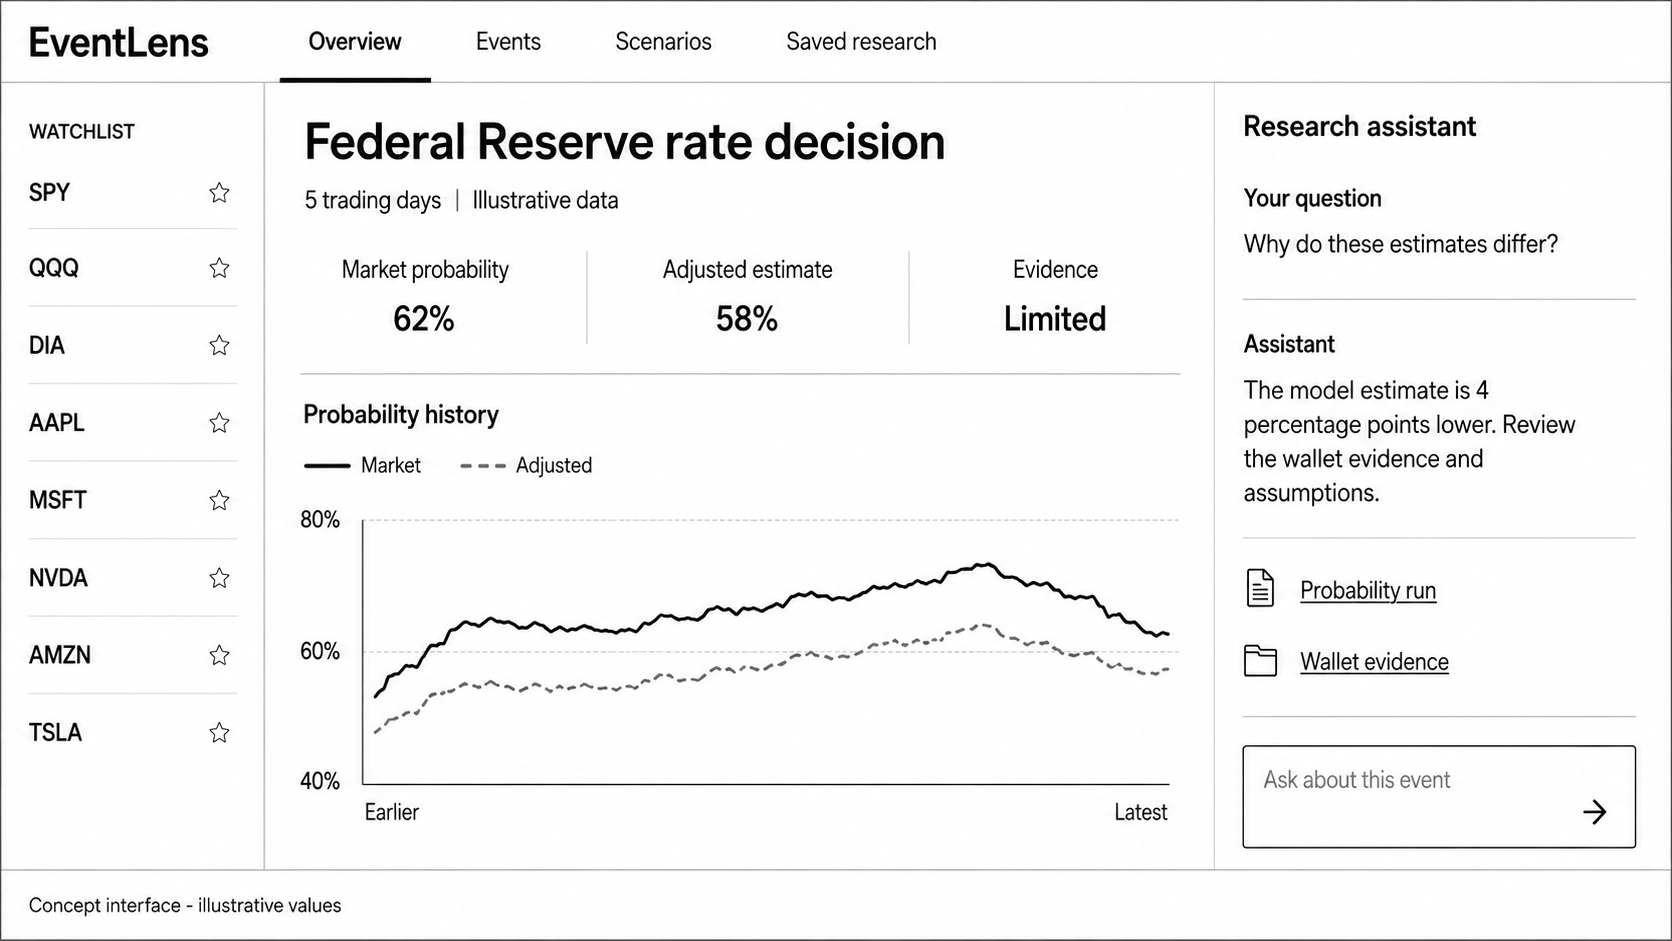
\includegraphics[width=\linewidth]{figures/overview-ui.png}
\caption{Overview concept: a watchlist, event probability comparison and contextual research assistant. All displayed values are illustrative.}
\label{fig:overview-ui}
\end{figure}
\begin{figure}[H]
\centering
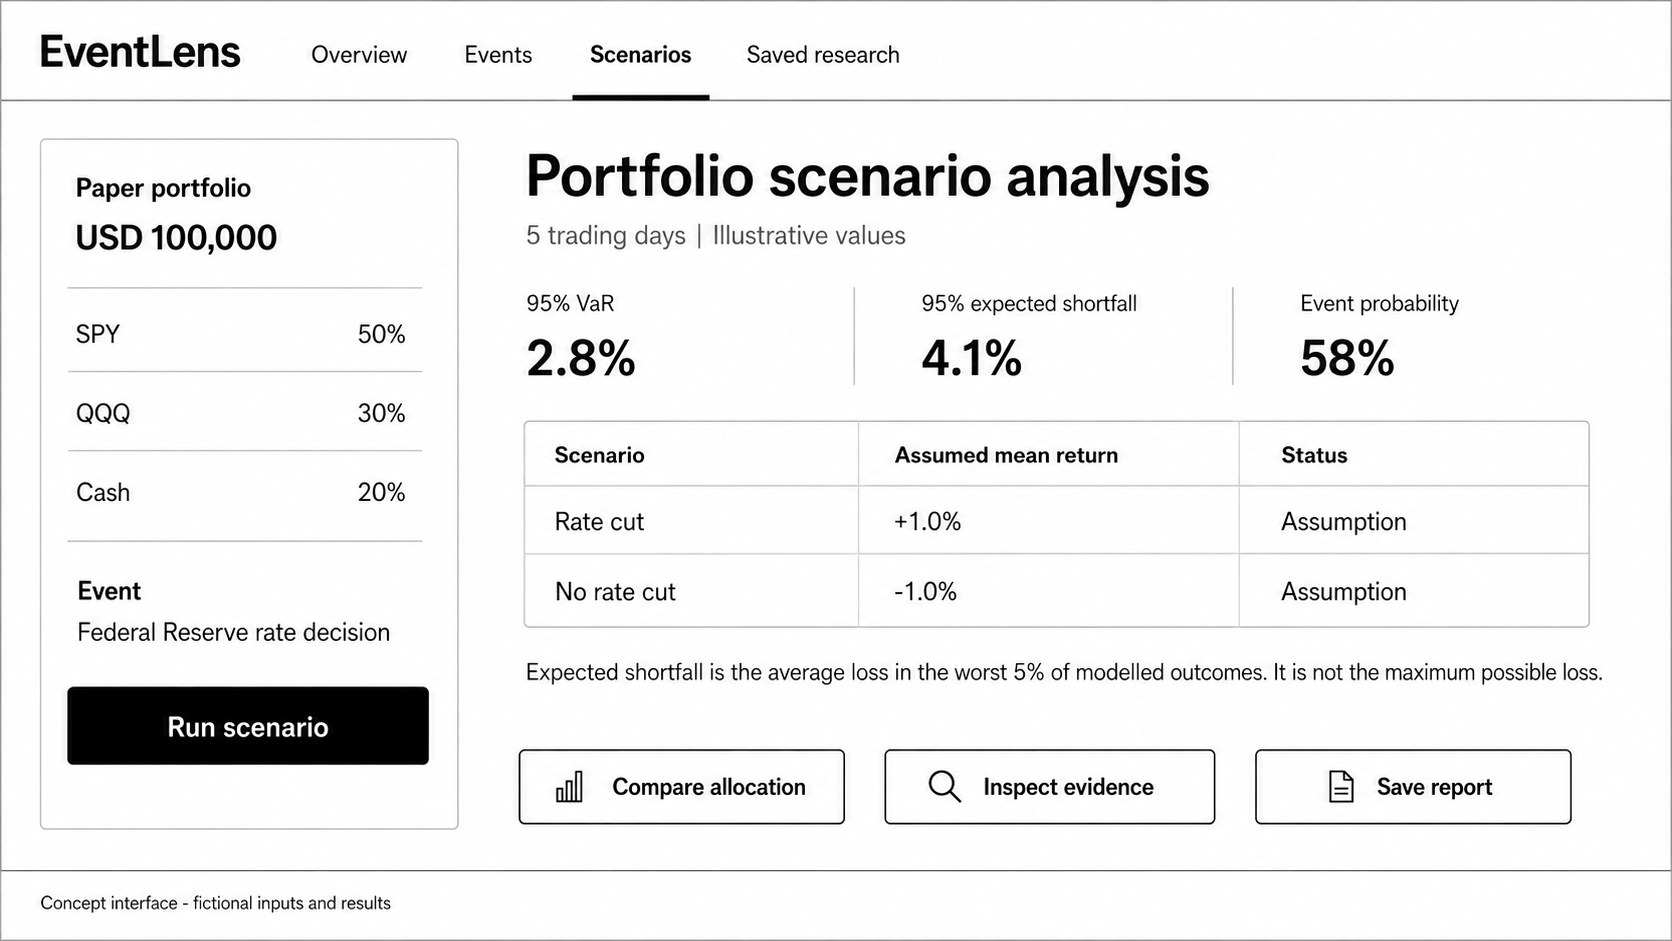
\includegraphics[width=\linewidth]{figures/scenario-ui.png}
\caption{Scenario concept: portfolio inputs, clearly labelled model outputs and visible assumptions. The user compares paper scenarios without placing orders.}
\label{fig:scenario-ui}
\end{figure}

\clearpage
\subsubsection{Three roles within one controlled workflow}
The proposed assistant will use three logical roles: an \textbf{event research agent} to find relevant evidence, an \textbf{analysis coordinator} to request approved calculations, and an \textbf{explanation agent} to present results in context. These roles can share one model and orchestration service in the MVP. A separate autonomous agent infrastructure is unnecessary.

\begin{figure}[H]
\centering
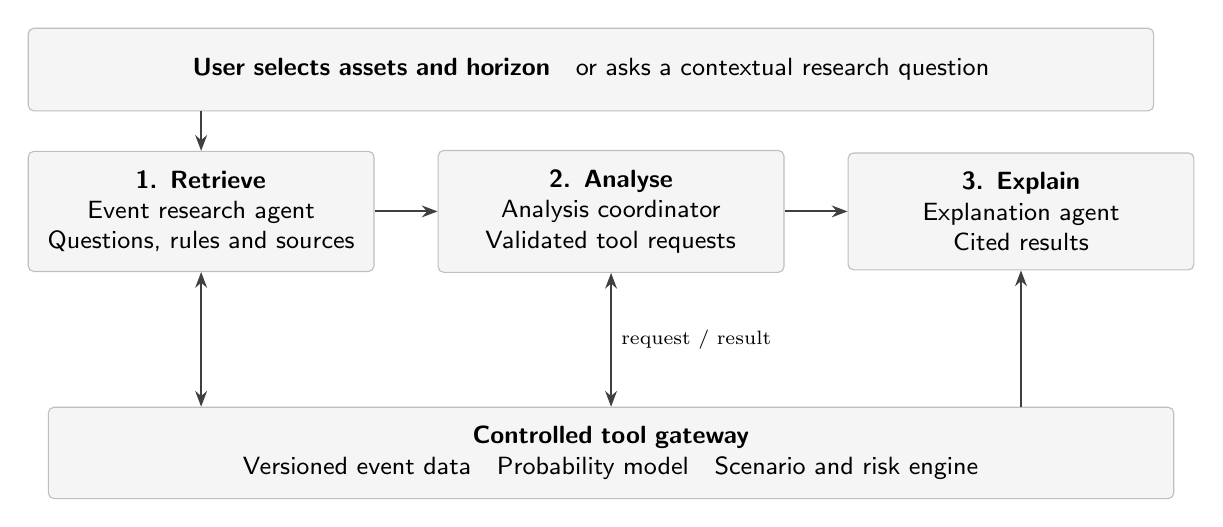
\begin{tikzpicture}[node distance=5mm and 8mm]
\node[flowbox,text width=13.8cm] (user) {\textbf{User selects assets and horizon}\quad or asks a contextual research question};
\node[flowbox,text width=3.9cm,below=of user.south west,anchor=north west] (research) {\textbf{1. Retrieve}\par Event research agent\par Questions, rules and sources};
\node[flowbox,text width=3.9cm,right=of research] (analysis) {\textbf{2. Analyse}\par Analysis coordinator\par Validated tool requests};
\node[flowbox,text width=3.9cm,right=of analysis] (explain) {\textbf{3. Explain}\par Explanation agent\par Cited results};
\node[flowbox,text width=13.8cm,below=17mm of analysis] (tools) {\textbf{Controlled tool gateway}\par Versioned event data\quad Probability model\quad Scenario and risk engine};
\draw[flowarrow] (user.south -| research.north)--(research.north);
\draw[flowarrow] (research)--(analysis);
\draw[flowarrow] (analysis)--(explain);
\draw[flowarrow,{Stealth[length=2mm]}-{Stealth[length=2mm]}] (research.south)--(research.south |- tools.north);
\draw[flowarrow,{Stealth[length=2mm]}-{Stealth[length=2mm]}] (analysis.south)--node[right,font=\scriptsize]{request / result}(tools.north);
\draw[flowarrow] (tools.north -| explain.south)--(explain.south);
\end{tikzpicture}
\caption{Proposed agent workflow. All quantitative results come from the same validated services used by the dashboard.}
\end{figure}

\subsubsection{From a question to a supported answer}
For ``How could the next rate decision affect my SPY and MSFT exposure?'', the assistant resolves the assets, horizon and analysis time. It retrieves an eligible event and proposes an event-to-asset explanation. Numerical responses must come from historical estimates or reviewed stress assumptions; generated text alone is not sufficient evidence.

The coordinator can call tools such as \texttt{find\_events}, \texttt{get\_wallet\_evidence}, \texttt{get\_probability}, \texttt{run\_scenario} and \texttt{compare\_allocations}. The gateway checks asset coverage, weights, units, data freshness and horizon compatibility. It returns structured values with sources, model versions and a research-run identifier. The explanation then links its numerical claims to those results and separates observations, estimates and assumptions \cite{lewis,yao}.

\subsubsection{Boundaries and review}
Users confirm changes to their paper inputs and can inspect assumptions before running a comparison. Researchers review new event-to-asset mappings and choose model versions using validation results. The agent cannot alter wallet labels, tune against the final test period, invent missing prices, calculate risk in prose or submit live orders. Market descriptions are treated as untrusted data, including any embedded instructions.

When evidence is incomplete, the assistant will identify the gap and offer a supported view, such as the raw probability. Tool traces and saved reports make answers reviewable. Evaluation will cover citations, numerical agreement, abstention, user understanding, response time and cost.

\clearpage
\subsubsection{Sources and their roles}
The data pipeline will combine three kinds of evidence: prediction-market information, public blockchain settlement records and conventional financial data. These sources serve different purposes. Polymarket matches orders off-chain and settles trades on-chain, so an order-book snapshot is not itself a blockchain record \cite{polymarketorder}.

\begin{table}[H]
\smalltable
\caption{Planned sources, with access decisions made during the feasibility audit.}
\begin{tabularx}{\linewidth}{@{}L{35mm}Y Y@{}}
\toprule\tablehead
\textbf{Source} & \textbf{Data to acquire} & \textbf{Use and limitation} \\
\midrule
Polymarket metadata API (Gamma) & Event definitions, rules, identifiers, outcome prices and available price history. & Define the forecast target and archive changes to mutable metadata \cite{polymarketdata}. \\
Polymarket CLOB and activity Data API & Bid/ask snapshots, liquidity and public wallet activity. & Measure market quality and candidate wallet flow. Historical book depth may need prospective collection. \\
Goldsky Polymarket datasets & Indexed fills, matched trades and relevant position records. & Targeted historical reconstruction, subject to version coverage and access cost \cite{goldsky}. \\
Polygon RPC & Transaction receipts, contract logs and block references. & Verify a stratified sample of settlements. Older state may require archival access. \\
Alpha Vantage or an approved equivalent & Daily equity/ETF prices, splits and dividends, with intraday data if available. & Proposed primary price-provider adapter. Adjusted daily data are a premium function. Coverage and academic-use terms must be checked \cite{alphavantage}. \\
Federal Reserve & Meeting dates, statements and announced rate decisions. & Establish announcement timing and validate event labels separately from platform resolution \cite{fed}. \\
\bottomrule
\end{tabularx}
\end{table}

\subsubsection{How on-chain data benefits EventLens}
Public settlement records link activity to addresses and outcome tokens \cite{polymarketorder}. EventLens will use these histories to measure historically informative wallets' directional exposure, agreement and concentration across covered events. Separating transfers and token lifecycle operations from purchases avoids treating every balance increase as a new prediction.

Users can trace contributions to recorded transactions, and researchers can check indexed data against chain receipts. Addresses represent pseudonymous accounts, not verified people or independent decision-makers. Comparing models with and without wallet features will test whether this Web3 evidence improves forecasts. Provenance alone does not establish skill.


\clearpage
\subsubsection{Turning source records into research inputs}
\begin{figure}[H]
\centering
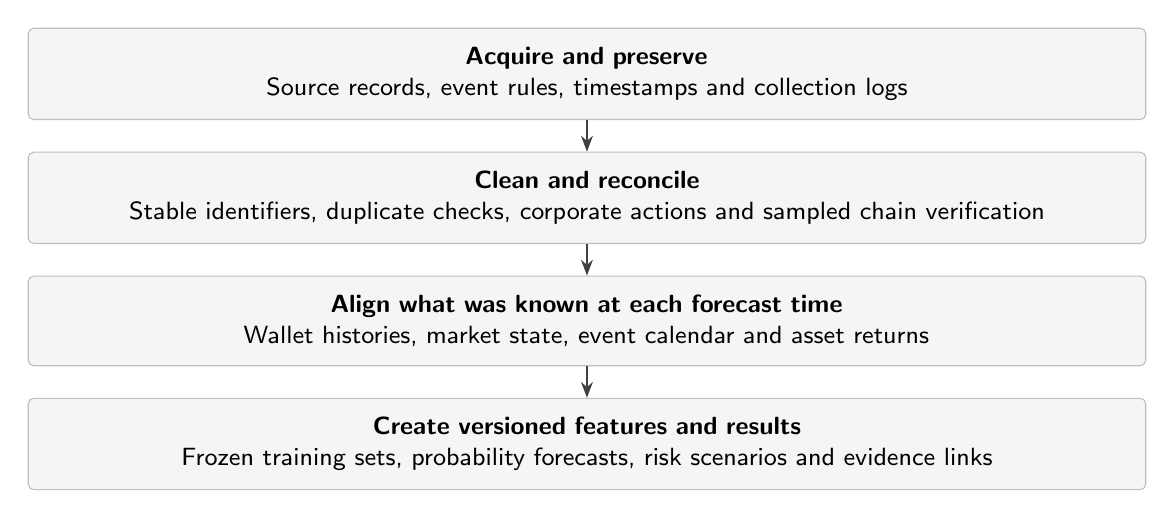
\begin{tikzpicture}[node distance=4mm]
\node[flowbox,text width=13.7cm] (raw) {\textbf{Acquire and preserve}\par Source records, event rules, timestamps and collection logs};
\node[flowbox,text width=13.7cm,below=of raw] (clean) {\textbf{Clean and reconcile}\par Stable identifiers, duplicate checks, corporate actions and sampled chain verification};
\node[flowbox,text width=13.7cm,below=of clean] (align) {\textbf{Align what was known at each forecast time}\par Wallet histories, market state, event calendar and asset returns};
\node[flowbox,text width=13.7cm,below=of align] (model) {\textbf{Create versioned features and results}\par Frozen training sets, probability forecasts, risk scenarios and evidence links};
\draw[flowarrow] (raw)--(clean);\draw[flowarrow] (clean)--(align);\draw[flowarrow] (align)--(model);
\end{tikzpicture}
\caption{Processing pipeline. Raw evidence is retained so each transformation can be checked and repeated.}
\end{figure}

\textbf{Preserve identifiers and time.} Each event is linked to its markets, outcome tokens and settlement records. Raw records retain source time, collection time and source version. Announcement time, platform resolution time and data-availability time remain separate. Historical records downloaded later are admissible only when their content can be shown to have existed at the forecast cut-off. Mutable current rankings are not historical features.

\textbf{Reconstruct activity consistently.} Wallet analysis retains both participant perspectives, while market volume counts the economic trade once. A transaction may contain several logs, so transaction hash alone is not a unique record key. We will use chain, transaction, log and contract identifiers and verify sampled amounts against Polygon receipts. Position reconstruction must account for transfers, splits, merges and redemptions as well as trades. Incomplete positions receive a quality flag.

\textbf{Align asset returns.} Timestamps will be normalised to UTC while retaining the US trading calendar, daylight-saving changes and after-hours announcements. Splits and dividends will be handled consistently. Future adjustments or revised data must not change historical features without a recorded version. Missing bars will be flagged rather than filled with zero returns. Stale probabilities will not be carried across an announcement as if newly observed.

\textbf{Make processing reproducible.} Immutable source snapshots and checksums will accompany cleaned tables and Parquet research files. Collectors will use retries, rate limits and checkpoints. Replaying the same batch must not duplicate records. Each model run stores the data manifest, configuration, code version and random seed, and the interface will expose coverage gaps through its evidence panel.

\clearpage
\subsubsection{Estimate the event probability}
We will begin with a raw probability based on the YES bid/ask midpoint, recording spread, depth and timestamp. When both outcome books are usable, their midpoints can be normalised for consistency. A missing or one-sided book will be flagged, not silently replaced by an unrelated latest trade.

A simple regularised logistic model will calibrate this estimate using earlier resolved events. The wallet-informed model will then add a small number of signals: overall directional flow, the flow of historically informative wallets and market-quality controls. Coefficients will be fitted on training data, rather than chosen to produce a desired adjustment. Beta calibration is a possible robustness check if justified by the sample \cite{kull}.

\subsubsection{Select and track informative wallets}
An informative wallet is an observed account whose earlier decisions contain information beyond the contemporaneous market price. Our first score will examine whether the wallet repeatedly chose the eventual outcome at informative prices, whether prices subsequently moved in its direction, and how broad its prior history was. Returns after fees will be a supporting diagnostic; profitable liquidity provision alone is not proof of forecasting skill.

Repeated fills will be consolidated into wallet--event decisions. Balanced YES and NO holdings will be distinguished from directional exposure. Scores based on few independent events will be pulled towards the population average, a technique called shrinkage. A provisional eligibility rule is ten earlier resolved events across at least three announcement dates, with five- and twenty-event thresholds checked in sensitivity analysis. If the history cannot support this rule, the wallet signal will be unavailable rather than assigned artificial confidence.

Wallet eligibility and scores will use only records available and outcomes resolved by each forecast cut-off. New activity updates exposure; newly resolved events update later scores. Frozen snapshots prevent today's successful wallets from being retrospectively selected for earlier tests.

Contributions combine earlier skill, direction, recency and capped size so one large wallet cannot dominate. Comparing total and eligible-wallet flow tests whether selection adds information. Profiles expose these components, timestamps, concentration and disagreement; new-wallet anomalies remain separate from historical skill.

\subsubsection{Link events to assets}
The event research agent may suggest that a rate decision matters to SPY or MSFT, but numerical impacts will come from matched historical event windows and conventional market controls. The mapping must account for surprise relative to the expectation already embedded in prices. Sparse asset-specific estimates will be pooled or replaced by explicitly reviewed stress ranges.

Wallet information may improve an event probability without improving an equity-risk forecast. The event-to-asset response is a separate estimate with its own uncertainty and evidence requirements.

Each mapping will retain its event definition, horizon, sample size, estimated response range and review status. A terminal YES/NO mixture will only be used when the economic announcement falls within the risk horizon. Otherwise the MVP will offer a compatible horizon or withhold that calculation. Correlated contracts from one meeting will not be treated as independent shocks.

\clearpage
\subsubsection{Explore portfolio scenarios and tail risk}
For a selected portfolio, the engine will combine the conditional return distributions for an event occurring (YES) and not occurring (NO). Let $p$ be the selected event probability, $\mu$ a mean portfolio return and $\sigma^2$ its variance over the same horizon. The key calculations are:
\begin{align}
\mu_{\mathrm{mix}} &= p\mu_{\mathrm{YES}}+(1-p)\mu_{\mathrm{NO}}, \\
\sigma^2_{\mathrm{mix}} &= p\sigma^2_{\mathrm{YES}}+(1-p)\sigma^2_{\mathrm{NO}}
 +p(1-p)(\mu_{\mathrm{YES}}-\mu_{\mathrm{NO}})^2.
\end{align}
The last term captures uncertainty about which outcome occurs. Consequently, a higher adverse-event probability can worsen expected loss without necessarily increasing variance. For multiple holdings, we will preserve cross-asset dependence when sampling returns, then apply the user's weights to each joint scenario.

The engine will report scenario returns, horizon volatility, a chosen loss-threshold probability, 95\% VaR and 95\% expected shortfall. VaR is a threshold, not the maximum loss. Expected shortfall will be calculated as the average of the worst 5\% of the weighted loss distribution, including fractional threshold mass where needed. We will use empirical or heavy-tailed scenarios and check sensitivity to the probability and asset-response assumptions.

Paper comparisons will hold the event and model version constant while comparing the current allocation with a user-selected reduction in a supported holding and a corresponding increase in cash. Weights must sum to one and remain non-negative. Any displayed benefit must be considered alongside turnover, transaction-cost assumptions and estimation uncertainty.

\subsubsection{Volatility Forecasting \& Delta-Hedged Trading Strategy Extension}

Once the on-chain-adjusted probability $p_{\text{adj}}$ is obtained, EventLens bridges prediction-market dynamics to traditional asset volatility through a dedicated Volatility Forecasting and Delta-Hedged Trading Strategy extension. This pipeline automates contract selection, feature extraction, volatility model fitting, and delta-hedged paper trading to evaluate the forecasting performance of on-chain signals.

\paragraph{Recurring event series and contract selection}
Polymarket serves as the sole source of prediction-market data for EventLens. The platform provides continuous tracking across recurring event families, including macroeconomic releases (e.g., FOMC rate decisions, CPI releases) as well as binary Polymarket contracts on equity index closing levels (e.g., S\&P 500 / NASDAQ daily and weekly target closes) and precious metals price targets (e.g., Gold and Silver closes).

To maintain temporal consistency across continuous volatility forecasting horizons, an automated contract selection engine identifies and locks onto the closest-to-expiry market contract for any chosen event family. When event resolutions overlap or liquidity is fragmented across multiple contracts, the selection engine filters for active contracts meeting minimum volume and bid-ask spread thresholds, continuously rolling to the next active contract upon resolution.

\paragraph{Feature engineering pipeline}
The feature extraction layer constructs point-in-time predictive signals derived from the adjusted probability $p_{\text{adj}}$ alongside raw market microstructure variables. Users are given interactive control to toggle and configure exogenous inputs depending on their desired baseline.

\begin{itemize}
    \item \textbf{Probability Signal Metrics}: Includes $p_{\text{adj}}$, raw probability $p_{\text{raw}}$, probability spread $(p_{\text{adj}} - p_{\text{raw}})$, model confidence bands, and probability jump/surprise signals ($\Delta p_{\text{adj}}$ measured over historical lookback windows up to the forecast cutoff).
    \item \textbf{User-Configurable Exogenous Baselines}: Allows optional inclusion of benchmark volatility proxies (e.g., VIX, MOVE) and historical realized volatility as regime controls.
\end{itemize}

\paragraph{Realized volatility forecasting models}
The extracted signals serve as exogenous features to forecast future realized volatility over standard horizons (e.g., 1-day, 5-day). The core target over $H$ trading days is defined as the sum of squared daily log returns:
\begin{equation}
RV_{t,H}=\sum_{h=1}^{H} r_{t+h}^{2}.
\end{equation}

EventLens implements three core volatility model structures:
\begin{itemize}
    \item \textbf{HAR-RV-X (Heterogeneous Autoregressive with Exogenous Signals)}: Extends the classical HAR-RV framework (which models realized volatility via daily, weekly, and monthly components) by adding linear exogenous terms for $p_{\text{adj}}$ and probability jump signals. Assumes a linear, multi-frequency structure for volatility persistence.
    \item \textbf{GARCH-X}: Incorporates exogenous prediction-market jump and log-odds signals directly into the conditional variance equation of a standard GARCH model. Assumes stationarity and clustering in conditional volatility returns.
    \item \textbf{Machine Learning Baselines (XGBoost / Random Forest)}: Non-linear tree ensemble models fitted on historical volatility features, probability spreads, and regime signals. Evaluated using standard robust loss functions such as QLIKE (Quasi-Likelihood) and Mean Squared Error (MSE) to prevent extreme volatility outliers from distorting model fitting.
\end{itemize}

\paragraph{Delta-hedged backtesting framework}
To demonstrate the practical utility of the forecasted realized volatility, EventLens runs an automated delta-hedged backtest. The backtest engine compares the model's forecasted realized volatility against current option-implied volatility (IV) from option market quotes to identify implied-versus-forecasted variance gaps. 

When a variance gap is detected, the strategy simulates a delta-neutral position (e.g., ATM options hedged continuously against the underlying asset) to harvest the variance risk premium. Costs, bid/ask spreads, hedge frequency, and execution assumptions are included. This simplified backtest framework provides the user with an intuitive evaluation of forecast performance, displaying backtested Sharpe ratios, maximum drawdowns, and simulated trade logs directly on the research dashboard.
\clearpage\subsection{Implementation}
\begingroup
\titlespacing*{\subsubsection}{0pt}{9pt}{4pt}
\setlength{\intextsep}{7pt}
\captionsetup{skip=4pt}
\renewcommand{\arraystretch}{1.08}
The implementation below is a proposed starting configuration. Named libraries, schemas and model settings will be explored during the feasibility stage.

\subsubsection{Application structure}
Next.js/React and TypeScript will use \href{https://tanstack.com/query/latest/docs/framework/react/overview}{TanStack Query} for fetching and job polling. FastAPI/Pydantic will validate JSON contracts \cite{nextjs,fastapi}. SQLAlchemy/Alembic will manage database access/migrations. A Python worker will collect data, fit models and run scenarios.



\subsubsection{API and frontend integration}
\begin{table}[H]
\smalltable
\caption{Proposed endpoints and compact Pydantic contracts.}
\begin{tabularx}{\linewidth}{@{}L{47mm}Y Y@{}}
\toprule\tablehead
\textbf{Endpoint} & \textbf{Input schema} & \textbf{Response schema} \\
\midrule
\texttt{GET /events} & asset, as\_of, cursor & events[], next\_cursor \\
\texttt{GET /wallets/\{address\}} & event\_id, as\_of & score, coverage, activity[] \\
\texttt{POST /analyses} & AnalysisRequest (below) & 202: job\_id, status \\
\texttt{GET /jobs/\{id\}} & job UUID & status, result?, error? \\
\texttt{GET /runs/\{id\}} & run UUID & metrics, units, as\_of, evidence[] \\
\texttt{POST /assistant/query} & session\_id, question, run\_id? & 202: job\_id, status \\
\bottomrule
\end{tabularx}
\end{table}
\textbf{AnalysisRequest:} event\_id: UUID, as\_of: UTC timestamp, horizon: $1|5|20$, holdings: [\{asset: string, weight: float\}]. Weights must be non-negative and sum to one. Invalid inputs return 422 with field errors. AssistantAnswer contains text, run IDs and citations. Cache keys include input and data/model versions. Stale or incomplete evidence is flagged.

\subsubsection{Data ingestion and storage}
HTTPX collectors will fetch incremental pages. Polars/PyArrow will preserve normalised Parquet evidence. Checkpoints, retries and unique source keys will support safe replay. Fills, transfers, splits, merges and redemptions will be reconciled, with sampled Polygon receipt checks.

\begin{table}[H]
\smalltable
\caption{Core physical schema. PK = primary key, FK = foreign key. Internal IDs use UUIDs.}
\begin{tabularx}{\linewidth}{@{}L{31mm}Y@{}}
\toprule\tablehead
\textbf{Table} & \textbf{Key fields and constraints} \\
\midrule
market\_snapshot & id PK, market\_id FK, observed\_at/collected\_at timestamps, price numeric(18,8), evidence\_uri text, source\_key text unique. \\
wallet\_score & id PK, address text, event\_id FK, cut\_off timestamp, score float, history\_count integer, version text. \\
analysis\_run & id PK, event\_id FK, request JSONB, snapshot\_ids JSONB, model\_version FK, seed integer, results JSONB. \\
model\_version & id text PK, estimator text, params JSONB, train\_cut\_off timestamp, artifact\_uri text. \\
job & id PK, run\_id FK nullable, kind/status text, attempts integer, heartbeat timestamp, error JSONB. \\
evidence\_chunk & id PK, event\_id FK, source\_uri text, body text, available\_at timestamp, embedding vector(384), embedding\_version text. \\
assistant\_session & id PK, owner\_id FK, summary text, context JSONB, updated\_at timestamp. \\
\bottomrule
\end{tabularx}
\end{table}
Market/time and wallet/event/cut-off indexes support dated lookups. Numeric results stay in SQL/Parquet. Embeddings support document retrieval only.

\clearpage
\subsubsection{Analytical pipeline}
\begin{table}[H]
\smalltable
\caption{Example feature spaces. Each row is constructed at an information cut-off $t$.}
\begin{tabularx}{\linewidth}{@{}L{28mm}Y L{38mm}@{}}
\toprule\tablehead
\textbf{Task / one row} & \textbf{Candidate features $X_t$} & \textbf{Target / output} \\
\midrule
Volatility / asset-date & Past 20-day mean $r^2$, raw event probability, adjusted minus raw probability & Future $RV_{t,H}$ for $H=1,5,20$ \\
Probability / event-date & Raw probability, spread, anonymous directional flow, eligible-wallet weighted flow & Resolved YES/NO label, then $p_{\mathrm{adj}}$ \\
Clustering / wallet-date & Turnover/capital, net YES--NO exposure, event concentration, typical holding duration & Behaviour group, with no outcome label \\
\bottomrule
\end{tabularx}
\end{table}

\begin{figure}[H]
\centering
% Generated synthetic values. Seed 42. No empirical research claims.
\def\regpoints{(0.2000,0.4631) (0.3130,0.2195) (0.4261,0.7284) (0.5391,0.8531) (0.6522,0.2383) (0.7652,0.4731) (0.8783,0.8955) (0.9913,0.8680) (1.1043,1.0190) (1.2174,0.8974) (1.3304,1.3924) (1.4435,1.4471) (1.5565,1.3554) (1.6696,1.6892) (1.7826,1.6100) (1.8957,1.3707) (2.0087,1.7446) (2.1217,1.5051) (2.2348,2.0252) (2.3478,1.8815) (2.4609,1.9282) (2.5739,1.8883) (2.6870,2.4243) (2.8000,2.1729)}
\def\regintercept{0.18668}
\def\regslope{0.73917}
\def\toyvar{3.93619}
\def\toyes{4.57566}
\expandafter\def\csname cluster0\endcsname{(0.1900,-0.6423) (0.2573,-0.5561) (0.2489,-0.5483) (0.3699,-0.6488) (0.1841,-0.6977) (0.2631,-0.4645) (0.2120,-0.7008) (0.1623,-0.5219) (0.2720,-0.5348) (0.1734,-0.5721) (0.2282,-0.5738) (0.2810,-0.5732) (0.2675,-0.5919) (0.2402,-0.5242) (0.1180,-0.6384) (0.1871,-0.6767)}
\expandafter\def\csname cluster1\endcsname{(0.7780,0.7294) (0.7307,0.6662) (0.6654,0.5098) (0.8130,0.6203) (0.8569,0.6452) (0.7721,0.4945) (0.8686,0.5270) (0.6979,0.4140) (0.7264,0.6097) (0.8114,0.6329) (0.7658,0.5690) (0.8500,0.5129) (0.8365,0.4706) (0.7710,0.5042) (0.7043,0.6084) (0.7624,0.5515)}
\expandafter\def\csname cluster2\endcsname{(0.5137,0.1336) (0.5266,0.0682) (0.4504,0.0704) (0.3619,-0.0937) (0.3874,-0.0397) (0.5080,-0.0287) (0.4535,0.2359) (0.4551,0.1685) (0.4146,0.0553) (0.4135,0.0393) (0.5388,-0.1273) (0.5104,0.1085) (0.4384,-0.0935) (0.4850,0.0165) (0.4963,0.0826) (0.5921,0.0513)}
\def\clustercentres{(0.2284,-0.5916) (0.7757,0.5666) (0.4716,0.0405)}

\begin{tikzpicture}
\begin{axis}[name=reg,width=5.2cm,height=4.4cm,scale only axis=false,
 title={\textbf{Regression}},title style={font=\small\sffamily},
 xlabel={Past 20-day mean $r^2$},ylabel={Next 5-day $RV$},
 label style={font=\scriptsize},tick label style={font=\scriptsize},
 xmin=0,xmax=3,ymin=0,ymax=3,xtick={0,1,2,3},ytick={0,1,2,3},
 axis lines=left,grid=major,grid style={gray!15},clip=false]
\addplot[only marks,mark=*,mark size=1.3pt,gray] coordinates {\regpoints};
\addplot[black,thick,domain=0:3]{\regintercept+\regslope*x};
\node[font=\tiny,anchor=north west] at (rel axis cs:0,1) {Units: $10^{-4}$};
\end{axis}
\begin{axis}[name=clust,at={(reg.east)},anchor=west,xshift=1.2cm,width=5.2cm,height=4.4cm,
 title={\textbf{Wallet clustering}},title style={font=\small\sffamily},
 xlabel={Turnover / capital per day},ylabel={Directional exposure},
 label style={font=\scriptsize},tick label style={font=\scriptsize},
 xmin=0,xmax=1,ymin=-1,ymax=1,xtick={0,.5,1},ytick={-1,0,1},axis lines=left,grid=major,grid style={gray!15}]
\addplot[only marks,mark=o,mark size=1.5pt,black] coordinates {\csname cluster0\endcsname};
\addplot[only marks,mark=triangle*,mark size=1.5pt,gray] coordinates {\csname cluster1\endcsname};
\addplot[only marks,mark=square*,mark size=1.4pt,black] coordinates {\csname cluster2\endcsname};
\addplot[only marks,mark=x,mark size=4pt,very thick,black] coordinates {\clustercentres};
\end{axis}
\begin{axis}[at={(clust.east)},anchor=west,xshift=1.2cm,width=5.2cm,height=4.4cm,
 title={\textbf{Scenario loss}},title style={font=\small\sffamily},
 xlabel={Portfolio loss (\%)},ylabel={Density},label style={font=\scriptsize},tick label style={font=\scriptsize},
 xmin=-3,xmax=6,ymin=0,ymax=.34,xtick={-2,0,2,4,6},ytick={0,.15,.3},axis lines=left,
 declare function={mix(\x)=.6*exp(-((\x-2)/1.4)^2/2)/(1.4*sqrt(2*pi))+.4*exp(-((\x+.5)/.8)^2/2)/(.8*sqrt(2*pi));}]
\addplot[draw=none,fill=gray!40,domain=\toyvar:6,samples=40]{mix(x)}\closedcycle;
\addplot[black,thick,domain=-3:6,samples=100]{mix(x)};
\draw[dashed] (axis cs:\toyvar,0)--(axis cs:\toyvar,.26);
\node[font=\tiny,anchor=east] at (axis cs:\toyvar,.28) {95\% VaR};
\draw[dotted] (axis cs:\toyes,0)--(axis cs:\toyes,.17);
\node[font=\tiny,anchor=west] at (axis cs:\toyes,.19) {ES};
\end{axis}
\end{tikzpicture}

\caption{Synthetic examples, not research results. A fitted line, wallet groups with centroid crosses, and a loss mixture with its worst 5\% shaded. ES is the mean loss in that tail.}
\end{figure}

\begin{table}[H]
\smalltable
\caption{Candidate implementations in \href{https://scikit-learn.org/stable/supervised_learning.html}{scikit-learn}. The team will explore all five techniques and retain models supported by validation.}
\begin{tabularx}{\linewidth}{@{}L{32mm}L{49mm}Y@{}}
\toprule\tablehead
\textbf{Technique} & \textbf{Estimator / role} & \textbf{Initial exploration} \\
\midrule
Linear regression & LinearRegression / variance & Recent-return baseline and event-augmented fit. \\
Logistic regression & LogisticRegression / probability & Regularisation strength and wallet-feature contribution. \\
SVM & SVC / outcome, SVR / variance & Linear or RBF kernel, $C$, gamma. Calibrate classifier scores chronologically. \\
MLP & MLPClassifier / MLPRegressor & One small hidden layer, e.g.\ 8 or 16 units, L2 penalty. \\
Clustering & StandardScaler + KMeans & Explore $k=2$--$5$, separation and stability across dated samples. \\
\bottomrule
\end{tabularx}
\end{table}

\begin{figure}[H]
\centering
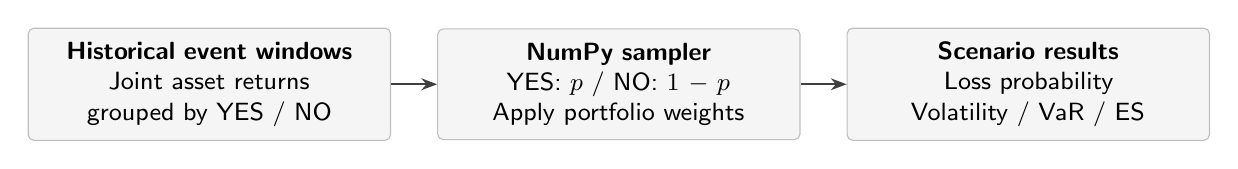
\begin{tikzpicture}[x=1cm,y=1cm,b/.style={flowbox,text width=4.25cm,font=\small\sffamily,inner sep=5pt,minimum height=1.35cm}]
\node[b] (a) at (0,0) {\textbf{Historical event windows}\\Joint asset returns\\grouped by YES / NO};
\node[b] (b) at (5.2,0) {\textbf{NumPy sampler}\\YES: $p$ / NO: $1-p$\\Apply portfolio weights};
\node[b] (c) at (10.4,0) {\textbf{Scenario results}\\Loss probability\\Volatility / VaR / ES};
\draw[flowarrow] (a)--(b);\draw[flowarrow] (b)--(c);
\end{tikzpicture}
\caption{Scenario execution preserves joint asset returns. The seed and evidence manifest are saved.}
\end{figure}
\textbf{Experiment controls.} Pipeline will fit scaling/imputation on training folds only. Chronological, event-grouped validation will purge overlapping targets, including for MLP tuning. Scores, clusters and probability fits use past data only. The regression baseline stays fixed. Clusters do not establish skill or ownership. Incomplete positions exclude affected features. Insufficient scenario evidence triggers an unavailable result or a labelled, reviewed stress assumption.

\clearpage
\subsubsection{Research assistant integration}
\href{https://docs.crewai.com/en/concepts/flows}{CrewAI Flows} is the proposed orchestrator. A typed Pydantic state will hold session\_id, event\_id, assets, horizon, as\_of, evidence IDs and run IDs. Three agent roles will work inside an explicit retrieve--calculate--explain flow. The workflow graph controls execution. Event--asset relationships will initially use relational joins, with knowledge-graph retrieval reserved for later exploration.

\begin{figure}[H]
\centering
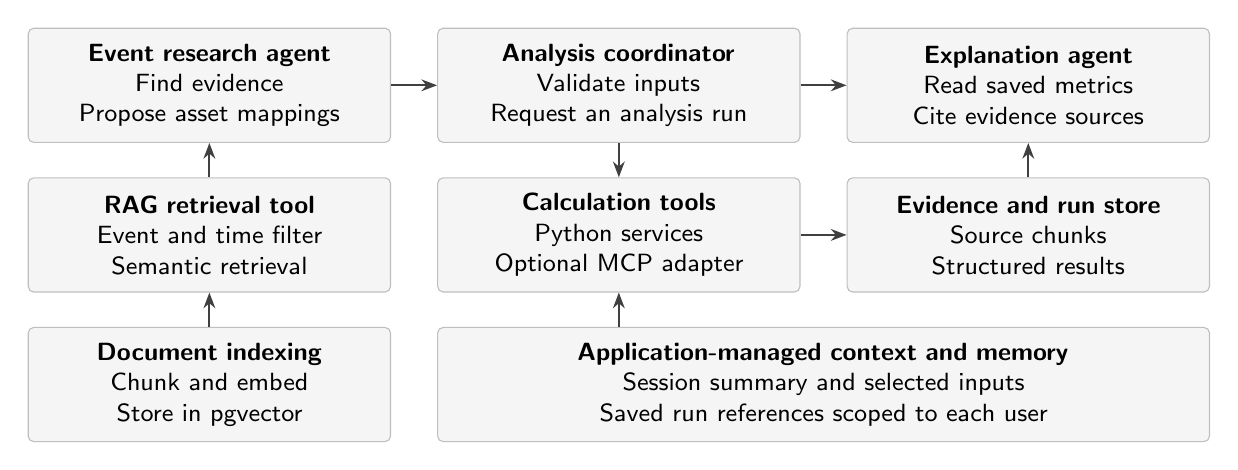
\begin{tikzpicture}[x=1cm,y=1cm,b/.style={flowbox,text width=4.25cm,font=\small\sffamily,minimum height=1.45cm,inner sep=5pt}]
\node[b] (r) at (0,0) {\textbf{Event research agent}\\Find evidence\\Propose asset mappings};
\node[b] (a) at (5.2,0) {\textbf{Analysis coordinator}\\Validate inputs\\Request an analysis run};
\node[b] (e) at (10.4,0) {\textbf{Explanation agent}\\Read saved metrics\\Cite evidence sources};
\node[b] (rag) at (0,-1.9) {\textbf{RAG retrieval tool}\\Event and time filter\\Semantic retrieval};
\node[b] (calc) at (5.2,-1.9) {\textbf{Calculation tools}\\Python services\\Optional MCP adapter};
\node[b] (res) at (10.4,-1.9) {\textbf{Evidence and run store}\\Source chunks\\Structured results};
\node[b] (emb) at (0,-3.8) {\textbf{Document indexing}\\Chunk and embed\\Store in pgvector};
\node[b,text width=9.45cm] (mem) at (7.8,-3.8) {\textbf{Application-managed context and memory}\\Session summary and selected inputs\\Saved run references scoped to each user};
\draw[flowarrow] (r)--(a);\draw[flowarrow] (a)--(e);
\draw[flowarrow] (emb)--(rag);\draw[flowarrow] (rag)--(r);
\draw[flowarrow] (a)--(calc);\draw[flowarrow] (calc)--(res);\draw[flowarrow] (res)--(e);
\draw[flowarrow] (mem.north -| a.south)--(calc.south);
\end{tikzpicture}
\caption{Proposed assistant workflow. Retrieved prose provides context. Typed calculation outputs provide numerical claims. New event--asset mappings require review before use.}
\end{figure}

\begin{table}[H]
\smalltable
\caption{Concrete retrieval, tool and memory design choices.}
\begin{tabularx}{\linewidth}{@{}L{27mm}Y@{}}
\toprule\tablehead
\textbf{Mechanism} & \textbf{Proposed implementation} \\
\midrule
RAG + embeddings & Archive event rules, official releases and reviewed mappings. Split into about 180 model-token chunks with 30-token overlap. Sentence Transformers \href{https://huggingface.co/sentence-transformers/all-MiniLM-L6-v2}{all-MiniLM-L6-v2} produces 384-dimensional embeddings. Store source, date and embedding version with every chunk. \\
Retrieval & \href{https://github.com/pgvector/pgvector}{pgvector} cosine search plus PostgreSQL keyword search. Merge ranked matches and return an initial top five. Filter by event, user access and information cut-off before ranking. Exact prices and positions come from SQL tools. \\
Function / tool use & CrewAI \href{https://docs.crewai.com/en/concepts/tools}{BaseTool} with Pydantic arguments: search\_evidence(query, event\_id, as\_of), get\_wallet\_evidence(address, event\_id, as\_of), run\_analysis(AnalysisRequest), get\_run(run\_id). Tools return evidence IDs, job IDs or typed results. \\
MCP option & A \href{https://docs.crewai.com/en/mcp/overview}{CrewAI MCP adapter} may expose the same approved functions to other clients. MCP is a tool interface, not a memory store. Direct Python tools are sufficient for the initial single deployment. \\
Context + memory & Load selected inputs, the latest six messages, a session summary, retrieved chunks and referenced results into a bounded prompt. Store owner-scoped summaries/preferences in PostgreSQL. Reload numerical facts from run IDs. Summaries never become research evidence. \\
\bottomrule
\end{tabularx}
\end{table}

\subsubsection{Deployment and reproducibility}
Docker Compose will run frontend, API, worker and PostgreSQL/pgvector services. A PostgreSQL job queue with retries and heartbeat expiry will recover interrupted work. Record prompts, tool traces, embedding/model versions and source manifests. Keep authenticated access, secrets, persistent volumes and backups. The assistant will stop after bounded tool calls, report missing evidence and preserve dashboard access when the hosted model fails.

\endgroup

\clearpage
\subsection{Testing}
Testing checks that the implementation is \emph{correct}, that the code and pipeline do what they are meant to do -- independently of whether the underlying research hypothesis turns out to be true.

\textbf{Data and pipeline tests.} Ingestion will be checked for schema validity, duplicate-free replay after an interrupted collection run, and reconciliation of a sample of collected records against source APIs and blockchain data. A point-in-time check will reject any feature or wallet history that uses information published after its forecast cut-off, since look-ahead leakage is the failure most likely to silently invalidate every downstream result without producing an obvious error. Corporate-action handling (splits, dividends) and timestamp normalization across time zones and daylight-saving changes will also be covered, since these are easy to get subtly wrong and hard to notice later.

\textbf{Calculation tests.} The probability model, wallet-scoring routine and the scenario/risk engine will be unit-tested against reference cases with known outputs: event probabilities of exactly zero and one, a missing asset, a one-sided or illiquid order book, and a singular or near-singular covariance matrix. API-level tests will enforce structural invariants -- portfolio weights non-negative and summing to one, horizons restricted to supported values, VaR and expected shortfall computed consistently with their definitions -- so that a broken invariant fails loudly rather than producing a plausible but incorrect result.

\textbf{Workflow and agent tests.} End-to-end tests will exercise the full path from event selection to a saved, shareable report, including stale or unavailable upstream data. Agent-specific tests will cover malformed or out-of-scope tool requests and adversarial instructions embedded in retrieved market or news text, since retrieved content is treated as untrusted data rather than instructions. The standing requirement is that every number shown to the user, including any number referenced by the AI assistant, traces back to a saved, versioned result rather than to generated text. This will itself be checked by a small set of tests that compare assistant output against the underlying stored result.

\textbf{Indicative metrics.} Pass/fail against the reference cases and invariants above, automated-test coverage of the ingestion and calculation modules, zero duplicate records after a replayed or interrupted collection run, and successful, byte-identical reproduction of a prior run's results from its stored data manifest, configuration and random seed.

\subsection{Evaluation}
Evaluation asks whether the finished system meets the objectives in Section~1.2.

\begin{table}[H]
\smalltable
\caption{How each objective will be evaluated (indicative and subject to refinement after the feasibility audit).}
\begin{tabularx}{\linewidth}{@{}L{20mm} L{42mm} Y@{}}
\toprule\tablehead
\textbf{Objective} & \textbf{Question} & \textbf{Indicative metric} \\
\midrule
Wallet identification & Does the smart-wallet score capture information beyond chance? & Backtested accuracy/Brier score vs.\ a label-shuffled baseline, with sensitivity to the eligibility threshold \\
Wallet-informed probability & Does wallet-weighting improve on the raw market price? & Brier score and log loss across the baseline ladder (raw price $\rightarrow$ +liquidity $\rightarrow$ +anonymous flow $\rightarrow$ +wallet signal) \\
Volatility forecasting & Do event features improve the same regression model? & MSE and QLIKE for the recent-return baseline and its augmented version on identical forecast dates \\
Related-event analysis & Do reviewed related events add information beyond the target event? & MSE and QLIKE for target-only versus target-plus-related-event features on identical forecast dates \\
Agent contribution & Does agent-assisted event selection improve over fixed rules? & Mapping precision and downstream forecast loss for rule-based, agent-assisted and hybrid configurations \\
Dashboard and assistant & Is the system usable, and does it stay evidence-linked? & Formative user study: task completion, numerical agreement between assistant and dashboard, correct abstention on insufficient data \\
\bottomrule
\end{tabularx}
\end{table}

\subsubsection{Experimental design}
Comparisons will use a chronological train/validation/test split, with each event's contracts and snapshots kept together and overlapping return windows purged at split boundaries, so that no test-period information leaks backward. The final test interval will remain untouched until the models and thresholds are fixed. Wallet scores, calibration and scenario inputs will use only information available as of each historical forecast time, matching the point-in-time discipline enforced in testing.

Predictive stability will also be reported across rolling and calendar subperiods. This will reveal whether an apparent improvement is persistent or concentrated in an earlier period. A signal that performs well initially but disappears in later unseen data will be reported as unstable rather than presented as general predictive value.

Given the likely small number of independent announcement dates, results will be reported with confidence intervals rather than as single numbers, and a broader macro sample would require a documented scope revision rather than an informal expansion mid-project. Multiple wallet-level significance tests will use a false-discovery correction rather than being read individually. A null result -- no measurable improvement from wallet or event signals -- is a valid and reportable outcome. Profitability is explicitly not a success criterion.

\subsubsection{Non-functional evaluation}
Beyond whether the numbers are right, the dashboard needs to be evaluated on qualities that determine whether it is actually usable for research in practice.

\textbf{Data freshness.} The interface implies near-real-time market and wallet state, so freshness itself needs to be measured rather than assumed: the lag between a Polymarket price update or a new on-chain fill and its appearance on the Overview and Event detail screens, and the lag between an FOMC announcement and the corresponding event being marked resolved. Data is never truly instantaneous once indexing and reconciliation are involved, so the target is a bounded, disclosed lag rather than zero latency -- the evidence panel already surfaces an as-of time for this reason, and that timestamp's accuracy is itself something to check, not just display.

\textbf{Responsiveness.} Interactive screens (watchlist, event detail, scenario studio) should remain usable while heavier jobs run in the background. Response time will be measured separately for cached/precomputed views versus a fresh scenario run or wallet backfill, since the latter are expected to be slower and are already designed to return a job identifier rather than block the interface.

\textbf{Reliability.} Uptime and error rate of the deployed prototype will be logged informally over the evaluation period (e.g., during the formative study and demonstration), along with the frequency of upstream provider failures (rate limits, stale feeds) and whether the system degrades to a clear "data unavailable" state rather than showing an unlabeled stale number.

\textbf{Cost.} Hosted-model and data-provider cost per research query and per full wallet backfill will be tracked, since this bounds how often scores can realistically be refreshed and how many events the assistant can be exercised against during the evaluation itself.

These are secondary to the correctness and research findings above, and will be reported descriptively (typical and worst-case figures) rather than against hard service-level targets, which would not be meaningful for a research prototype at this scale.

Success requires reproducible data and experiment configuration, a controlled baseline comparison, a tested risk engine, and a usable, evidence-linked interface. Positive, negative and null findings will all be reported. Exact sample sizes, thresholds and the final participant count will be confirmed once the data-feasibility audit (Section~2.1) fixes what history is actually available.

\pagechapter{Project Planning}
\subsection{Division of Work}
Franklin, Anthony, Owen and Sunny will work across four tracks, each with a lead and a reviewer. Named ownership remains to be agreed. All members will contribute to literature review, reporting and presentations.

\begin{table}[H]
\smalltable
\caption{Proposed work allocation, with named ownership to be recorded by the team.}
\begin{tabularx}{\linewidth}{@{}L{36mm}Y Y@{}}
\toprule\tablehead
\textbf{Track} & \textbf{Responsibility} & \textbf{Deliverable} \\
\midrule
Data and blockchain & Source adapters, collection, reconciliation and quality reporting. & Versioned dataset and coverage report. \\
Probability research & Wallet scoring, calibration, baseline comparisons and leakage controls. & Reproducible probability experiments. \\
Scenarios and risk & Asset-response estimates, volatility, tail risk and reference tests. & Deterministic risk engine and application study. \\
Product and AI & Backend integration, frontend, agent tools and deployment. & Integrated dashboard and user evaluation. \\
\bottomrule
\end{tabularx}
\end{table}

Git will hold code, experiment configuration and separate LaTeX section files for collaborative editing. Generated files and secrets stay out of version control. Weekly reviews and an issue tracker will record owners, dependencies, meeting decisions and experiment changes.

\subsection{GANTT Chart}
The schedule is relative to project commencement and will be aligned with course dates. Data feasibility comes first; interface work starts with sample data to identify integration problems early.

\begin{table}[H]
\smalltable
\caption{Planning baseline. Shaded cells indicate the main work period.}
\begin{tabularx}{\linewidth}{@{}Y*{6}{>{\centering\arraybackslash}p{11mm}}@{}}
\toprule\tablehead
\textbf{Workstream} & \textbf{1--4} & \textbf{5--8} & \textbf{9--12} & \textbf{13--16} & \textbf{17--20} & \textbf{21--24} \\
\midrule
Scope, literature and feasibility & \cellcolor{navy!22} & & & & & \\
Collection and reconciliation & \cellcolor{navy!22} & \cellcolor{navy!22} & \cellcolor{navy!22} & & & \\
Wallet and probability models & & \cellcolor{navy!22} & \cellcolor{navy!22} & \cellcolor{navy!22} & & \\
Event mapping and risk engine & & & \cellcolor{navy!22} & \cellcolor{navy!22} & \cellcolor{navy!22} & \\
Interface and AI integration & & \cellcolor{navy!22} & \cellcolor{navy!22} & \cellcolor{navy!22} & \cellcolor{navy!22} & \\
Evaluation and user study & & & & & \cellcolor{navy!22} & \cellcolor{navy!22} \\
Report and reproducibility & \cellcolor{navy!10} & \cellcolor{navy!10} & \cellcolor{navy!10} & \cellcolor{navy!10} & \cellcolor{navy!22} & \cellcolor{navy!22} \\
\bottomrule
\end{tabularx}
\end{table}

\textbf{Milestones.} Week 2: initial access and scope decision. Week 7: a versioned dataset and reconciliation report. Week 12: first raw-price, anonymous-flow and wallet-flow comparison. Week 18: working scenarios and risk calculations. Week 22: integrated evaluation and user tasks. Week 24: final report, demonstration and reproducibility package. Failed feasibility gates will narrow the model or coverage before optional work begins.

\pagechapter{Hardware and Software Requirements}
\subsection{Hardware Requirements}
The initial models and API-hosted language model do not require a local GPU. Development can be carried out on standard personal computers, with a modest shared server for scheduled collection and the demonstration.

\begin{table}[H]
\smalltable
\caption{Proposed hardware provision.}
\begin{tabularx}{\linewidth}{@{}L{32mm}Y Y@{}}
\toprule\tablehead
\textbf{Resource} & \textbf{Minimum provision} & \textbf{Preferred provision} \\
\midrule
Developer computer & Four-core CPU and 8\,GB RAM & 16\,GB RAM for concurrent local services. \\
Storage & 30\,GB free disk space & Approximately 100\,GB SSD space for bounded historical data. \\
Shared server & Local demonstration if necessary & 2--4 vCPU and 8--16\,GB RAM, subject to measured workload. \\
Network & Stable internet connection & Reliable access for collectors, hosted models and remote collaboration. \\
\bottomrule
\end{tabularx}
\end{table}

A self-hosted Polygon node is outside the initial scope. Hosted RPC and targeted indexed data will be used for collection and verification. Database and raw-data storage must persist across application updates and be backed up regularly.

\subsection{Software Requirements}
\begin{table}[H]
\smalltable
\caption{Required software and external services.}
\begin{tabularx}{\linewidth}{@{}L{32mm}Y Y@{}}
\toprule\tablehead
\textbf{Category} & \textbf{Software or service} & \textbf{Purpose} \\
\midrule
Runtime & Python and Node.js & Research services, collectors and web application. \\
Application & FastAPI, Pydantic, Next.js, React and TypeScript & Validated backend APIs and interactive interface. \\
Data and modelling & PostgreSQL, Parquet, Polars/Pandas, NumPy and scikit-learn & Storage, processing and initial statistical models. \\
External services & Polymarket APIs, Goldsky, Polygon RPC, equity data and hosted LLM & Event evidence, asset histories and research assistance. \\
Quality and deployment & Pytest, browser tests, Docker and Docker Compose & Automated verification and reproducible deployment. \\
Collaboration & Git, issue tracker and LaTeX & Source control, task allocation and shared documentation. \\
\bottomrule
\end{tabularx}
\end{table}

External costs may include adjusted equity histories, indexed blockchain access, archival RPC, a hosted language model and server hosting. The team will set a spending cap after checking sample data and provider terms during the feasibility stage. A paid historical options dataset is not required for the core project. Software dependencies, model versions and configuration will be recorded to support reproducibility.

\pagechapter{References}
% Selected references retained from the Word draft, with current source documentation.
\begingroup
\small
\setstretch{1.04}
\begin{thebibliography}{99}
\setlength{\itemsep}{7pt}
\bibitem{atanasov} 
  Atanasov, P., Rescober, P., Stone, E., Swift, S. A., Servan-Schreiber, E., Tetlock, P., Ungar, L., \& Mellers, B. (2017). ``Distilling the Wisdom of Crowds: Prediction Markets vs. Prediction Polls. Management Science, 63(3), 691--706. \href{https://doi.org/10.1287/mnsc.2015.2374}{https://doi.org/10.1287/mnsc.2015.2374}
\bibitem{akey} Akey, Pat and Gregoire, Vincent and Harvie, Nicolas and Martineau, Charles, ``Who Wins and Who Loses In Prediction Markets? Evidence from Polymarket (March 18, 2026). \href{http://dx.doi.org/10.2139/ssrn.6443103}{http://dx.doi.org/10.2139/ssrn.6443103}
\bibitem{chen} 
  Chen, Y., Chu, C.-H., Mullen, T., \& Pennock, D. M. (2005). ``Information markets vs. opinion pools: an empirical comparison. EC '05 : \textit{Proceedings of the 6th ACM Conference on Electronic Commerce} : Vancouver, Canada, June 5--8, 2005, 58--67. \href{https://doi.org/10.1145/1064009.1064016}{https://doi.org/10.1145/1064009.1064016}

\bibitem{wolfers2004} J. Wolfers and E. Zitzewitz, ``Prediction Markets,'' \textit{Journal of Economic Perspectives}, 18(2), pp. 107--126, 2004. \href{https://doi.org/10.1257/0895330041371321}{doi:10.1257/0895330041371321}.
\bibitem{wolfers2006} J. Wolfers and E. Zitzewitz, ``Interpreting Prediction Market Prices as Probabilities,'' NBER Working Paper 12200, 2006. \href{https://doi.org/10.3386/w12200}{doi:10.3386/w12200}.
\bibitem{brier} G. W. Brier, ``Verification of Forecasts Expressed in Terms of Probability,'' \textit{Monthly Weather Review}, 78(1), pp. 1--3, 1950.
\bibitem{gneiting} T. Gneiting and A. E. Raftery, ``Strictly Proper Scoring Rules, Prediction, and Estimation,'' \textit{Journal of the American Statistical Association}, 102(477), pp. 359--378, 2007. \href{https://doi.org/10.1198/016214506000001437}{doi:10.1198/016214506000001437}.
\bibitem{gomez} R. G\'omez-Cram, Y. Guo, T. I. Jensen and H. Kung, ``Prediction Market Accuracy: Crowd Wisdom or Informed Minority?'' SSRN Working Paper 6617059, 2026. Working paper, not peer reviewed. \href{https://doi.org/10.2139/ssrn.6617059}{doi:10.2139/ssrn.6617059}.
\bibitem{Oliven} 
  Oliven, K., \& Rietz, T. A. (2004). ``Suckers Are Born but Markets Are Made: Individual Rationality, Arbitrage, and Market Efficiency on an Electronic Futures Market.'' \textit{Management Science}, 50(3), 336--351. \href{https://doi.org/10.1287/mnsc.1040.0191}{doi:10.1287/mnsc.1040.0191}.
\bibitem{victor} F. Victor, ``Address Clustering Heuristics for Ethereum,'' \textit{Financial Cryptography and Data Security}, pp. 617--633, 2020. \href{https://doi.org/10.1007/978-3-030-51280-4_33}{doi:10.1007/978-3-030-51280-4\_33}.
\bibitem{mackinlay} A. C. MacKinlay, ``Event Studies in Economics and Finance,'' \textit{Journal of Economic Literature}, 35(1), pp. 13--39, 1997.
\bibitem{rockafellar} R. T. Rockafellar and S. Uryasev, ``Optimization of Conditional Value-at-Risk,'' \textit{Journal of Risk}, 2(3), pp. 21--41, 2000.
\bibitem{andersen} T. G. Andersen, T.
\bibitem{manski} Manski, C. F. (2006). ``Interpreting the predictions of prediction markets. Economics Letters, 91(3), 425--429. \href{https://doi.org/10.1016/j.econlet.2006.01.004}{https://doi.org/10.1016/j.econlet.2006.01.004}.
\bibitem{patton} A. J. Patton, ``Volatility Forecast Comparison Using Imperfect Volatility Proxies,'' \textit{Journal of Econometrics}, 160(1), pp. 246--256, 2011. \href{https://doi.org/10.1016/j.jeconom.2010.03.034}{doi:10.1016/j.jeconom.2010.03.034}.
\bibitem{gao} 
  Gao, J., Wang, Z., Wu, W., \& Yu, D. (2025). ``Price Interpretability of Prediction Markets: A Convergence Analysis. Operations Research, 73(1), 157--177. \href{https://doi.org/10.1287/opre.2022.0417}{https://doi.org/10.1287/opre.2022.0417}.


\end{thebibliography}
\clearpage
\section*{References (continued)}
\begin{thebibliography}{99}
\setcounter{enumiv}{11}
\setlength{\itemsep}{7pt}
\bibitem{lewis} P. Lewis et al., ``Retrieval-Augmented Generation for Knowledge-Intensive NLP Tasks,'' \textit{Advances in Neural Information Processing Systems}, 2020. \href{https://papers.nips.cc/paper_files/paper/2020/hash/6b493230205f780e1bc26945df7481e5-Abstract.html}{Proceedings and paper}.
\bibitem{yao} S. Yao et al., ``ReAct: Synergizing Reasoning and Acting in Language Models,'' \textit{ICLR}, 2023. \url{https://arxiv.org/abs/2210.03629}.
\bibitem{kull} M. Kull, T. M. Silva Filho and P. Flach, ``Beta Calibration: A Well-Founded and Easily Implemented Improvement on Logistic Calibration for Binary Classifiers,'' \textit{AISTATS}, pp. 623--631, 2017. \url{https://proceedings.mlr.press/v54/kull17a.html}.
\bibitem{polymarketorder} Polymarket, ``Order Lifecycle,'' documentation, accessed 5 September 2026. \url{https://docs.polymarket.com/concepts/order-lifecycle}.
\bibitem{polymarketdata} Polymarket, ``Market Data Overview,'' documentation, accessed 5 September 2026. \url{https://docs.polymarket.com/market-data/overview}.
\bibitem{goldsky} Goldsky, ``Indexing Polymarket with Goldsky,'' documentation, accessed 5 September 2026. \url{https://docs.goldsky.com/chains/polymarket}.
\bibitem{alphavantage} Alpha Vantage, ``API Documentation,'' including Daily Adjusted and corporate-action data, accessed 5 September 2026. \url{https://www.alphavantage.co/documentation/}.
\bibitem{fed} Board of Governors of the Federal Reserve System, ``Meeting Calendars and Information,'' accessed 5 September 2026. \url{https://www.federalreserve.gov/monetarypolicy/fomccalendars.htm}.
\bibitem{fastapi} FastAPI, ``Features,'' documentation, accessed 5 September 2026. \url{https://fastapi.tiangolo.com/features/}.
\bibitem{nextjs} Next.js, ``Server and Client Components,'' documentation, accessed 5 September 2026. \url{https://nextjs.org/docs/app/getting-started/server-and-client-components}.
\end{thebibliography}
\endgroup

\pagechapter{Appendix A: Meeting Minutes}

\subsection{Minutes of the 1st Project Meeting}

\textbf{Date:} 8 August 2026 (Saturday) \\
\textbf{Time:} 21:00 \\
\textbf{Place:} Zoom \\
\textbf{Present:} All members \\
\textbf{Absent:} None \\
\textbf{Recorder:} Sze Wang Cheong

\textbf{1. Approval of minutes} \\
There were no minutes to approve, as this was the first formal group meeting.

\textbf{2. Report on progress} \\
2.1 All members had reviewed the FYP proposal template and familiarised themselves with the submission requirements. \\
2.2 The group discussed the overall timeline and key milestones leading up to the proposal deadline.

\textbf{3. Discussion items} \\
3.1 The group agreed a structured timeline before the proposal submission: idea-sharing on 16 August; buffer sessions on 22 and 29 August; internal deadline (draft to communication tutor) on 3 September; review of tutor comments on 6 September; soft submission deadline on 10 September; hard submission deadline on 11 September. \\
3.2 The objective of the next meeting (16 August) was defined: each member would prepare and share project ideas, with the group deciding on a final topic by the end of that meeting.

\textbf{4. Goals for the coming month} \\
4.1 All members to prepare project ideas for the next meeting. \\
4.2 The group to keep to the agreed timeline so the internal draft is ready for tutor review by 3 September.

\textbf{5. Meeting adjournment and next meeting} \\
The meeting was adjourned at 21:12. The next meeting was scheduled for 21:00 on 16 August 2026, via Zoom.

\clearpage
\subsection{Minutes of the 2nd Project Meeting}

\textbf{Date:} 16 August 2026 (Sunday) \\
\textbf{Time:} 21:00 \\
\textbf{Place:} Zoom \\
\textbf{Present:} Anthony, Sunny, Owen, Franklin \\
\textbf{Absent:} None \\
\textbf{Recorder:} Team representative

\textbf{1. Approval of minutes} \\
The minutes of the 1st meeting (8 August 2026) were reviewed and approved.

\textbf{2. Report on progress} \\
2.1 All members had researched candidate FinTech, Web3 and quantitative-trading topics as scheduled. \\
2.2 All members prepared proposal ideas to present at this meeting.

\textbf{3. Discussion items} \\
3.1 Each member presented candidate directions: Anthony proposed several crypto/quant concepts, including cross-exchange arbitrage, an on-chain whale-tracking agent, a crypto risk-management framework and a market-anomaly-detection agent; Sunny proposed an end-to-end quant platform with an NLP module to translate strategy descriptions into backtestable code; Owen supported Sunny's direction, citing WorldQuant Brain as an industry reference; Franklin proposed an on-chain smart-wallet tracking system on Polymarket (Polygon) using a scoring model to detect informed trading. \\
3.2 The team agreed the project should be product-centric rather than strategy-centric, to keep a strong engineering and system-design scope. \\
3.3 The team noted the NLP-backtesting idea risked being too general and hard to backtest reliably for crypto/Web3 dynamics. \\
3.4 The team reviewed the feasibility of Franklin's Polymarket proposal, noting existing open-source tools already demonstrate reliable extraction of Polymarket on-chain data. \\
3.5 The team reached consensus on a unified direction: a Web3 intelligence system that ingests on-chain Polymarket data, identifies smart-wallet activity on relevant prediction markets, and translates those signals into insights for financial and equity markets (e.g.\ macro risk indicators).

\textbf{4. Goals for the coming week} \\
4.1 All members to research the methodology and architecture needed for the Polymarket intelligence platform (data sources, APIs, on-chain indexing and signal mapping). \\
4.2 All members to prepare detailed technical inputs for the draft proposal ahead of the internal deadline on 3 September.

\textbf{5. Meeting adjournment and next meeting} \\
The meeting was adjourned at 22:56. The next meeting was scheduled for 21:00 on 22 August 2026, via Zoom, to discuss system methodology and data-pipeline architecture.

\clearpage
\subsection{Minutes of the 3rd Project Meeting}

\textbf{Date:} 22 August 2026 (Saturday) \\
\textbf{Time:} 21:00 \\
\textbf{Place:} Zoom \\
\textbf{Present:} All members \\
\textbf{Absent:} None \\
\textbf{Recorder:} Team representative

\textbf{1. Approval of minutes} \\
The minutes of the 2nd meeting (16 August 2026) were reviewed and approved.

\textbf{2. Report on progress} \\
2.1 Members had used AI assistance to generate an initial full draft of the proposal (Overview, Objectives and Methodology) based on the team's prior discussions and research. \\
2.2 The draft was found to be substantially over length relative to the expected proposal size.

\textbf{3. Discussion items} \\
3.1 The team reviewed the proposed user workflow: a user selects a supported market category (e.g.\ a Federal Reserve rate-cut event), the system applies smart-wallet identification to derive an adjusted event probability, and an optional simple backtest of a volatility relative-value strategy is run on the result. \\
3.2 The team discussed the intended MVP dashboard: user-selected event categories, intermediate outputs (smart wallets, adjusted event probability) and final outputs (volatility and risk metrics such as Value at Risk). \\
3.3 The team clarified the role of the LLM agent: summarising smart-wallet evidence for the user, mapping a user's watchlist or portfolio to relevant Polymarket events, and offering context-appropriate suggestions once the user has entered their holdings. \\
3.4 The team confirmed all on-chain and market data would be sourced from Polymarket's API, including its central limit order book. \\
3.5 Referring to the FYP grading rubric (approximately 60\% objectives/methodology/background, 30\% organisation/clarity/presentation, 10\% planning and timeline), the team agreed the draft needed significant shortening, targeting roughly 10--15 pages, with the Design and Application subsection cut most aggressively. \\
3.6 The team discussed collaborative tooling for the LaTeX draft (Overleaf's per-project collaborator limits versus a Git-based workflow) and agreed to continue evaluating options. \\
3.7 The team agreed to request a consultation with the supervisor (Prof.\ Shuai Wang) ahead of submission, proposing Monday afternoon or Tuesday morning as candidate slots.

\textbf{4. Goals for the coming week} \\
4.1 Anthony to shorten the Introduction (overview and objectives). \\
4.2 Owen and Franklin to jointly shorten the Design and Application sections. \\
4.3 The remaining member to shorten the Testing and Evaluation section. \\
4.4 Franklin to email the supervisor to arrange a consultation slot before the internal deadline.

\textbf{5. Meeting adjournment and next meeting} \\
The meeting was adjourned. The next meeting was scheduled for 21:00 on 29 August 2026, via Zoom.

\clearpage
\subsection{Minutes of the 4th Project Meeting}

\textbf{Date:} 29 August 2026 (Saturday) \\
\textbf{Time:} 21:00 \\
\textbf{Place:} Zoom \\
\textbf{Present:} Anthony, Sunny, Owen, Franklin (Sunny joined shortly after the meeting began) \\
\textbf{Absent:} None \\
\textbf{Recorder:} Team representative

\textbf{1. Approval of minutes} \\
The minutes of the 3rd meeting (22 August 2026) were reviewed and approved.

\textbf{2. Report on progress} \\
2.1 Members had continued drafting their assigned sections following the shortening exercise agreed at the previous meeting.

\textbf{3. Discussion items} \\
3.1 The team revisited smart-wallet identification in more depth: given the limited history available on Polymarket (approximately three years) and the absence of a labelled dataset, the team agreed to first define rule-based labels (e.g.\ a historical win-rate threshold) and then train a model on these labels so that new, previously unseen wallets can also be scored. \\
3.2 The team discussed mapping the adjusted event probability to asset volatility, identifying GARCH-family models as a candidate approach for incorporating the adjusted probability as an input feature, while noting this mapping step has less data per event than the wallet-scoring step and needs a simpler, more robust design. \\
3.3 The team agreed to narrow the initial asset universe to a small set of index-tracking ETFs, which carry less idiosyncratic risk and are easier to forecast, before considering individual equities in a later phase. \\
3.4 The team clarified that the machine-learning components (wallet scoring, probability-to-volatility mapping) and the LLM research agent (event-to-asset relevance and user-facing explanation) are complementary rather than overlapping, so the design satisfies the project's AI requirement without redundancy. \\
3.5 The team discussed two possible uses for the volatility output -- portfolio risk management versus an actively traded volatility strategy -- and agreed to describe both directions in the proposal while prioritising the risk-management framing, since the primary target user is a retail investor rather than a derivatives trader. \\
3.6 The team agreed to source on-chain settlement data via Polygon RPC, in addition to Polymarket's own API for event metadata, to keep the project's Web3 focus; initial event coverage will prioritise finance/macroeconomics and politics/geopolitics categories over sports or other categories. \\
3.7 The team reviewed the FYP table of contents and grading rubric and split the remaining proposal-writing workload by section among the four members, agreeing to draft independent sections individually first and reconvene to jointly resolve the more interdependent Design and Methodology content. \\
3.8 The team noted an open question requiring further work: how to weight and aggregate multiple related Polymarket bets into a single adjusted volatility estimate for a given asset.

\textbf{4. Goals for the coming week} \\
4.1 All members to continue drafting their assigned proposal sections. \\
4.2 Members to individually explore a small proof-of-concept calculation for the probability-to-volatility aggregation step, to compare approaches at the next meeting. \\

\textbf{5. Meeting adjournment and next meeting} \\
The meeting was adjourned. The next meeting was scheduled ahead of the internal deadline of 3 September 2026, date and time to be confirmed.
\end{document}
